\begin{frame}{Perspectives}
Ce qui (n') a (pas) été réussi
Sacrifices faits (système opérationelle)
Problèmes rencontrés (NP-complétude)
Forces et faiblesses du sysème
Pistes à suivre pour une suite éventuelle
Évaluation du système à faire
\end{frame}

\begin{frame}{Perspectives}{Un treillis de concepts en mémoire ?}
\begin{block}{Le contexte}
Un contexte est un triplet $(G,M,I)$ avec
\begin{itemize}
\item $G$ l'ensemble des objets
\item $M$ l'ensemble des attributs
\item $I \in G*M$ l'ensemble des relations
\end{itemize}
On pourrait donc utiliser la mémoire sémantique comme contexte pour la création d'un treillis de concepts.
\end{block}
\end{frame}

\begin{frame}{Perspectives}{Un treillis de concepts en mémoire ?}
\begin{block}{Utile ?}
\begin{itemize}
\item Abstraction supplémentaire
\item Travail sur des ensembles de formes (RPBS)
\end{itemize}
\end{block}
\end{frame}

\begin{frame}{Perspectives}{Un treillis de concepts en mémoire ?}
\begin{block}{Exemple (concret)}
\begin{columns}[t]
	\begin{column}{0.5\textwidth}
	\only<3>{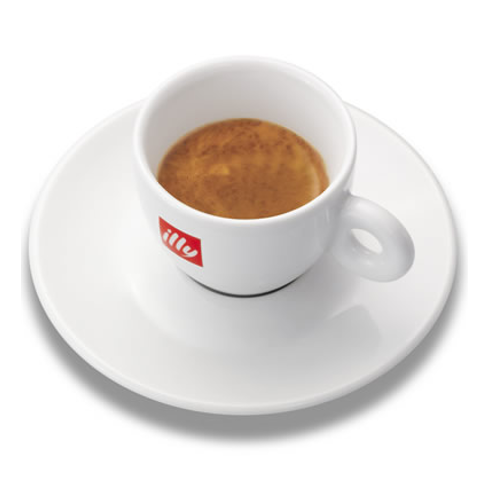
\includegraphics[width=0.5\textwidth]{img/conclusion/espresso_tmp}}
	\uncover<4->{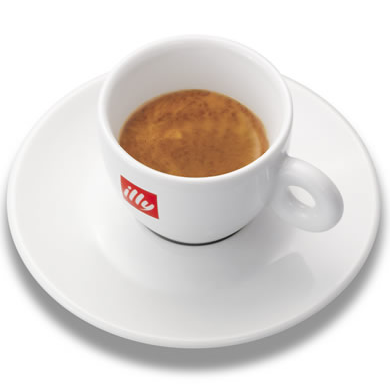
\includegraphics[width=0.5\textwidth]{img/conclusion/espresso}}
	\\
	\only<5>{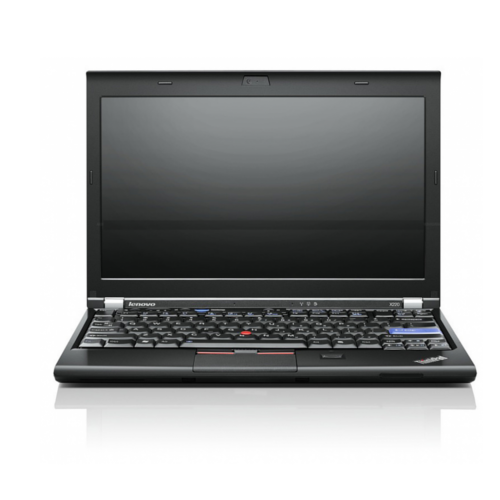
\includegraphics[width=0.5\textwidth]{img/conclusion/ordi_tmp}}
	\uncover<6->{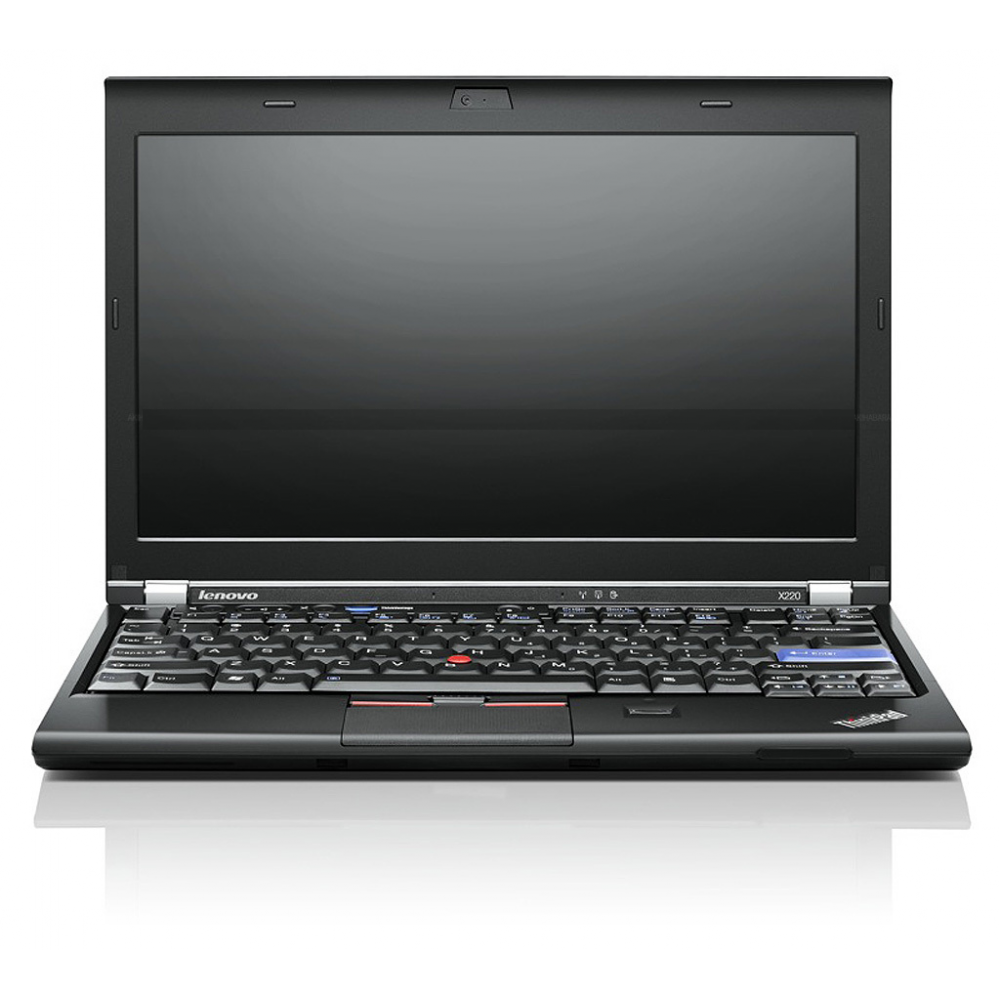
\includegraphics[width=0.5\textwidth]{img/conclusion/ordi}}
	\end{column}
	\begin{column}{0.5\textwidth}
	\only<7>{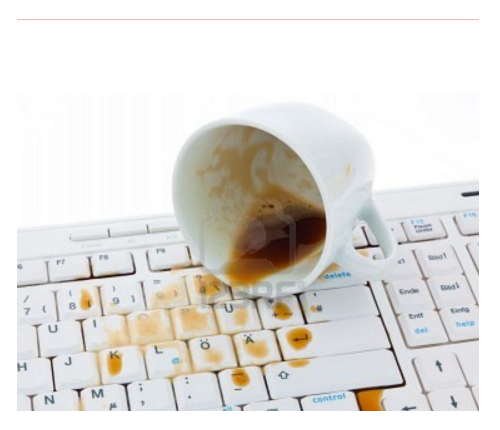
\includegraphics[width=0.7\textwidth]{img/conclusion/cafe_renverse_tmp}}
	\only<8->{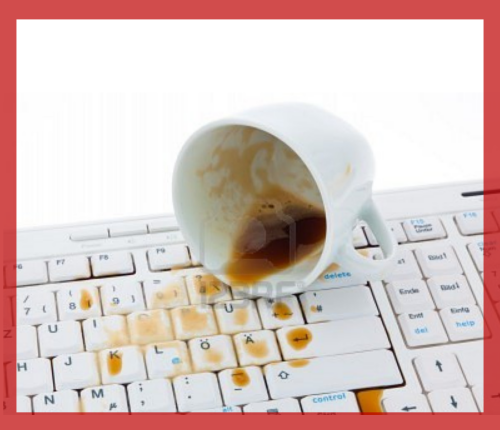
\includegraphics[width=0.7\textwidth]{img/conclusion/cafe_renverse}}
	\end{column}
\end{columns}
\end{block}
\end{frame}